%\documentclass[french]{beamer}
\documentclass[aspectratio=169]{beamer}
\usepackage[utf8]{inputenc}
\usepackage[T1]{fontenc}
\usepackage{lmodern}
\usepackage{amsmath, amssymb}
\usepackage{babel}

\usepackage{eurosym}
%\usepackage{unicode-math}
\setbeamertemplate{footline}[frame number]

\definecolor{rouge}{HTML}{DD0000}

%Pour le TITLEPAGE

\title{Appel à projet}
\subtitle{Mardi 7 mars 2023}
\date{}
\author[N.P. - A.M. - P.T.]{Nicolas Papazoglou, Alexis Martin \& Pierre Toussaint}
\institute[ENSEA]{ENSEA}

\usetheme{ensea}  

\AtBeginSection[]
{
	\begin{frame}{Plan}
		\tableofcontents[currentsection]
	\end{frame}
}

\AtBeginSubsection[]
{
   \begin{frame}
    	\tableofcontents[currentsection,currentsubsection]
   \end{frame}
}

\begin{document}

\begin{frame}
	\titlepage
\end{frame}

\begin{frame}{Appel à projet}
\begin{minipage}{0.49\textwidth}
	\begin{itemize}
		\item Porteurs du projet : Alexis Martin, Nicolas Papazoglou, Pierre Toussaint,
		\item Demande budgétaire : 64 HETD,
		\item Budget (DEE) : 400-500\euro/maquette,
		\item Activités concernées : enseignements d'électrotechnique et d'automatique.
	\end{itemize}
\end{minipage}
\begin{minipage}{0.49\textwidth}
	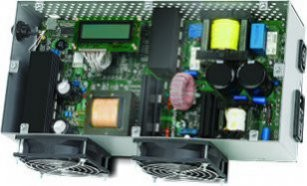
\includegraphics[scale=0.6]{figures/inverter.jpeg} 
\end{minipage}
\center \href{https://github.com/DBXYD/AAP_ENSEA_Inverter}{Lien github}
\end{frame}

%********************** OBJECTIFS ******************************
\begin{frame}{Contexte}
\begin{itemize}
	\item Maquette de TP : onduleur triphasé,
	\item TP en 3eme année (Enseignements d'électrotechnique et d'automatique) : 
	\begin{itemize}
	\item [AEI\_3121] Commande numérique directe de dispositifs
	\item [ESE\_3745] Actionneur et automatique appliquée
	\item [MSC\_3805] Systèmes d'Acquision et de commande
	\end{itemize}
	\item 12 maquettes obsolète Powermodule MC1L 3-Phase (Microchip) : 
	\item Pannes récurentes :
	\begin{itemize}
		\item Perte de temps pour les étudiants,
		\item Recherche de panne et réparation par les professeurs,
		\item Boite noire pour les étudiants.		
	\end{itemize}
\end{itemize}
\end{frame}

\begin{frame}{Objectif : Réalisation maquette pédagogique}
	Objectifs : 
	\begin{enumerate}
		\item Une maquette fiable pour les TPs d'électrotechnique et automatique \\
		$\rightarrow$ Gain en temps et en autonomie pour les étudiants,
		\item Feedback automatique en fonction des erreurs détectées, \\
		$\rightarrow$ Gain en autonomie pour les étudiants, possibilité de travail hors séance sans supervision d'un professeur,
		\item Projet open-source (disponible sur \href{https://github.com/DBXYD/AAP_ENSEA_Inverter}{github}),
		\item Compréhension globale possible par les étudiants, application de l'ensemble de leurs cours dans une maquette,
		\item Création modulaire, réutilisable dans d'autres cours/projets, 
		\item Evolution possible à d'autres enseignements (buck/boost, 4Q, brushless, moteurs synchrones, asservissement, etc...),
		\item Maintenance facile et rapide.
	\end{enumerate}
\end{frame}

\begin{frame}{Travail à effectuer}
\begin{enumerate}
	\item Cahier des charges (déjà effectué),
	\item Schéma d'architecture (déjà effectué),
	\item Choix des composants (disponibles et actuels pour une maintenibilité la plus longue possible),
	\item Prototypage et tests unitaires électriques,
	\item Réalisation software et tests complets,
	\item Réalisation mécanique (boitier),
	\item Intégration complète,
	\item Documentation (\href{https://github.com/DBXYD/AAP_ENSEA_Inverter}{github}).
\end{enumerate}
\end{frame}

\begin{frame}{Travail déjà effectué : Cahier des charges}
\begin{itemize}
	\item Onduleur triphasé 60V / 15A,
	\item Protections surtensions et surintensités,
	\item Commande de mise sous tension,
	\item Commande UART,
	\item Utilisable en commande ``brushless'' :  entrées position ``hall'' ,
	\item Utilisable en commande vectorielle ou MCC : entrée position ``encoder'',
	\item Protection alimentation non réversible : module ``freinage'',
	\item Vérification des temps morts,
	\item Mesure de courants (hall) dans les 3 phases + entrée,
	\item Mesure de tension dans les 3 phases + entrée,
	\item Alimentation externe secteur,
	\item Affichage erreurs, intensité PWM (affiche externe),
	\item Sorties mesures de courants et PWMs,
	\item Boitier,
	\item Tenue thermique,
	\item Isolation galvanique.
\end{itemize}
\end{frame}

\begin{frame}{Travail déjà effectué : Schéma d'architecture}
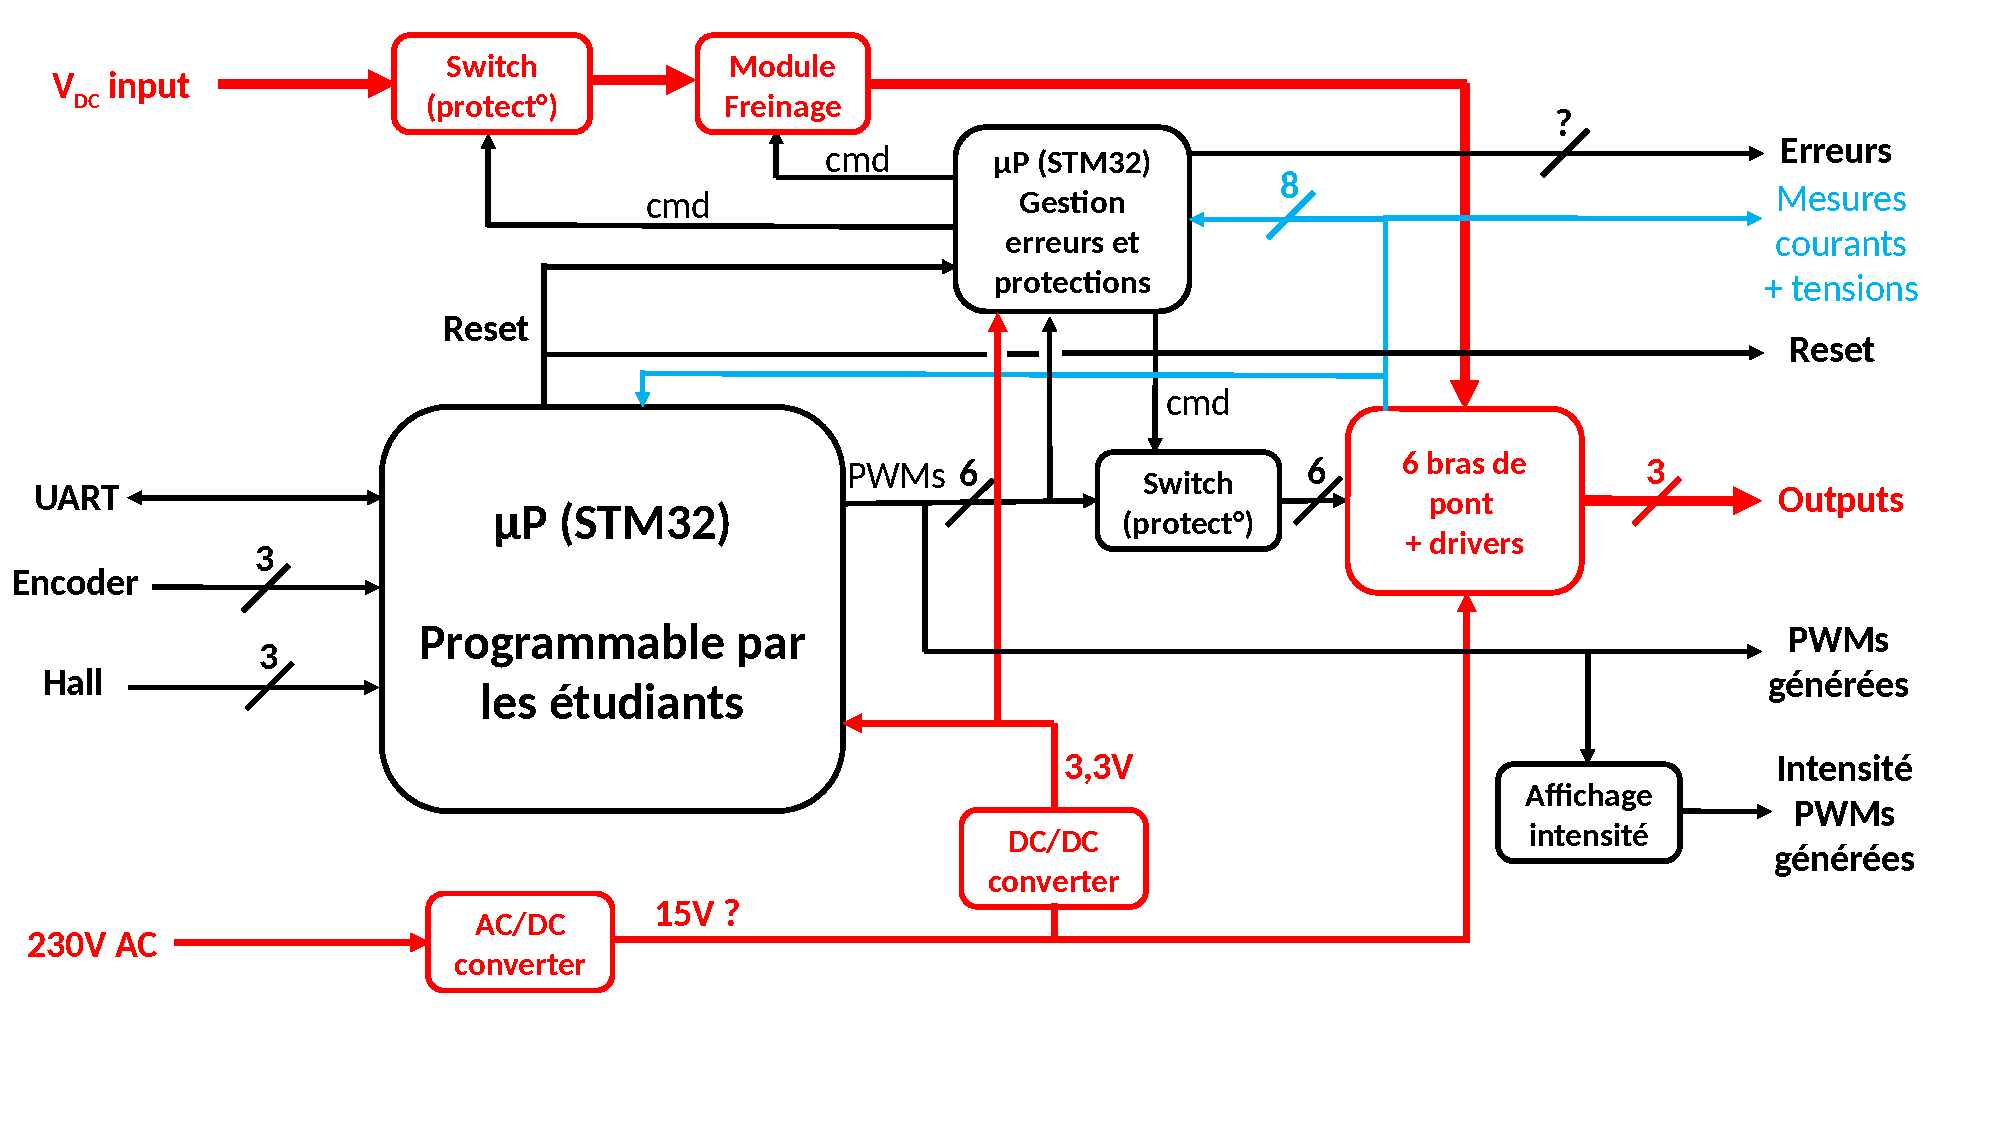
\includegraphics[width=\linewidth]{figures/Schema_architecture.pdf} 
\end{frame}

\begin{frame}{Dead-line et rémunération}
\begin{itemize}
	\item Prototype fonctionnel pour la rentrée de septembre 2023,
	\item Rémunération demandée : 64 HETD.
\end{itemize}

\end{frame}

\end{document}